\chapter{Estado del arte}

\section{Ingeniería del Software}

En esta sección voy a describir las herramientas que se usarán en este proyecto así como la justificación del uso de cada una. Todas están enfocadas para lograr las mejores prácticas de la metodología DevOps.

\subsection{Lenguaje elegido}

El lenguaje que he elegido para la realización de este proyecto ha sido Python, por ser muy fácil de aprender y además tiene un gran número de librerías para ciencia de datos.

\subsection{Gestor de dependencias}

El gestor de dependencias es una herramienta muy útil hoy en día para poder manejar las dependencias de una aplicación o un proyecto de forma sencilla, usando las órdenes del mismo. Además nos permite instalar todas las librerías usando únicamente una orden. Esto claramente ayuda a mantener la reproducibilidad de la aplicación ya que facilita bastante la ejecución de la misma aplicación en otra máquina (como por ejemplo en el entorno de Integración continua, en la máquina de entrenamiento de modelos o en la que desplegaremos un microservicio). En Python, los dos principales gestores de dependencias son \enquote{Pipenv} y \enquote{Poetry}.Ambas herramientas gestionan por debajo un entorno virtual aislado que contiene las dependencias instaladas.

\subsubsection*{Pipenv}

Pipenv se define como una herramienta que apunta a traer todo lo mejor del mundo del empaquetado al mundo Python \cite{pipenv}. Usa un fichero con sintaxis TOML para registrar las dependencias cuyo nombre es Pipfile.

\subsubsection*{Poetry}

Poetry es una herramienta cuya popularidad está creciendo un montón actualmente en la comunidad de Python. Es utilizada únicamente para manejar las dependencias de cualquier proyecto de forma muy sencilla. Además, cuenta con una documentación muy buena y clara \cite{poetry}.

\subsubsection*{Comparación de ambas herramientas}

Para comparar ambas herramientas para el manejo de dependencias, voy a utilizar el tiempo que tardan en instalar las librerías usando el fichero \textit{lock}. Las librerías que he usado como dependencias han sido \textit{PyTorch} y \textit{FastAPI} y de dependencias de desarrollo \textit{pylint} y \textit{pytest}. En la siguiente tabla se pueden ver los resultados:

\begin{table}[h]
\begin{tabular}{|c|c|c|}
\hline
                     & \textbf{Pipenv} & \textbf{Poetry} \\ \hline
\textbf{Ejecución 1} & 31,938          & 22,009          \\ \hline
\textbf{Ejecución 2} & 38,528          & 23,068          \\ \hline
\textbf{Ejecución 3} & 33,63           & 23,111          \\ \hline
\textbf{Ejecución 4} & 35,452          & 21,407          \\ \hline
\textbf{Ejecución 5} & 33,406          & 20,901          \\ \hline
\textbf{Media}       & 34,59           & 22,10           \\ \hline
\end{tabular}
\centering
\caption{Tiempo (medido en segundos) que tarda cada herramienta en instalar las dependencias anteriores.}
\label{tab:poetryvspipenv}
\end{table}

Como se puede ver en el Cuadro \ref{tab:poetryvspipenv}, Poetry es siempre más rápido que Pipenv, por lo tanto usaré Poetry para manejar las dependencias del proyecto. Además me gustaría añadir que en el momento del testeo, intenté instalar la librería \textit{black}, pero Pipenv me dió problemas, cosa que con Poetry no pasó. He hecho el test de tiempo debido a que necesito que se instalen las dependencias lo más rápido posible para que la Integración Continua dure lo menos posible en ejecutarse y para que se despliegue rápido la aplicación, ya que la instalación de dependencias es casi siempre lo que más tarda.

\subsection{Gestor de tareas}

Para seguir ayudando con la reproducibilidad del proyecto, necesitamos un gestor que contenga las órdenes necesarias para testear o arrancar la aplicación o lanzar el entrenamiento de modelos. Esto nos permite que nuestro proyecto se pueda ejecutar en otra máquina de forma sencilla, ejecutando una sola orden que ya lo hace todo por nosotros. Poetry no trae por defecto ningún gestor de tareas, al contrario que Pipenv que sí lo trae. Pero por suerte, existe una herramienta que nos añade un task manager en Poetry llamada \textit{Poethepoet}. Esta herramienta nos permite lanzar una tarea tan solo escribiendo \textit{poe $<taskname>$} \cite{poethepoet}.

\subsection{Plataforma de CI/CD}

La finalidad de esta plataforma es ejecutar los tests y realizar el despliegue cada vez que se produzca un incorporación de código al repositorio de GitHub. Se usará para controlar los cambios en el código. En la CI, lo que hace es ejecutar los tests para comprobar que todo funcione bien. Si la CI tiene éxito, los cambios se aprueban y se combinan en el repositorio compartido y se despliega la aplicación en la máquina destino. Esto sería así en DevOps, pero en MLOps tenemos que entrenar los modelos antes de desplegarlos, por lo cuál el workflow se hace un poco más complejo.

\begin{figure}[h]
	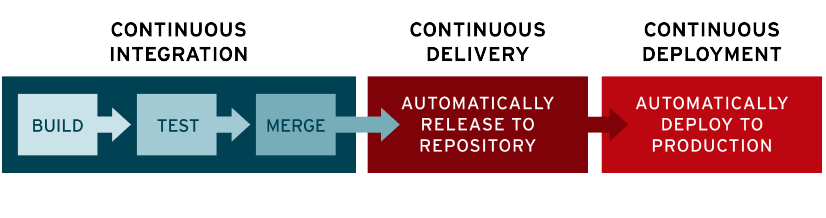
\includegraphics[scale=0.4]{imagenes/03_Estado_del_arte/ci-cd-flow.png}
	\centering
	\caption{Flujo de trabajo CI/CD. \cite{cicd}}
\end{figure}

Casi todas las plataformas de CI/CD tienen un plan de pago pero también tienen un plan gratuito. Mi criterio al seleccionar una plataforma de CI/CD concreta es gastar el menor dinero posible. Por ejemplo Travis, una plataforma que antes era gratuita y es muy rápida, otorgan ahora 10.000 créditos de los cuales, debido al uso que le di en una asignatura, solo me quedan 1650, por lo que esta plataforma queda descartada. En el caso de CircleCI, otorga 2.500 créditos gratis al mes, lo cual limitaría el número de subidas de código que puedo realizar en un mes y no me convence demasiado.\newline

Existen algunas plataformas gratuitas como por ejemplo Shippable, pero es demasiado lenta. GitHub Actions también es gratuita para repositorios públicos, como es el caso por lo que estaría interesante usarlo para comprobaciones básicas del repositorio, como por ejemplo comprobar la presencia de archivos importantes del mismo o comprobar la ortografía del README.\newline

Una plataforma a la que seguro le daré uso será Jenkins, tal vez una de las plataformas de CI/CD más populares escrita en Java. Esta plataforma es muy configurable y además dispone de un montón de plugins desarrollados por la comunidad que añaden un montón de utilidades. Para hacerlo funcionar, tenemos que instalarlo en un computador, por lo que sería necesario una instancia en alguna plataforma cloud para tenerlo disponible el mayor tiempo posible o incluso se podría ejecutar en una Raspberry Pi, lo único que necesitamos para que funcione es una Máquina Virtual Java. En mi caso tengo 150\$ en la plataforma AWSEducate, por lo que podría desplegar una instancia con Jenkins estando disponible el mayor tiempo posible sin problemas.\newline

Todas las plataformas anteriores disponen de un fichero de configuración que se almacena en el repositorio en el que hay que describir la secuencia de órdenes para poder ejecutar los tests o hacer el despliegue, además de especificar el contenedor en el que ese ejecuta, versiones del lenguaje, etc.

\subsection{Framework para MLOps}

Lo que necesito de un framework para MLOps es que registre los experimentos realizados (hiperparámetros usados y resultados obtenidos) y además nos facilite la reproducibilidad de los mismos, es decir, que se obtengan los mismos resultados independientemente de la máquina/entorno en el que se ejecuten.\newline

Existe un framework llamado SnapperML que facilita todo lo anterior. Permite almacenar los hiperparámetros de los modelos en formato YAML, además de tener un control de la estocasticidad (recoge información sobre la semilla utilizada para los diferentes generadores de números aleatorios). También permite el \textit{tracking} de experimentos usando \textit{MLFlow}, una herramienta que permite registrar métricas, hiperparámetros y artefactos y nos permite acceder a ellos a través de una interfaz web bastante intuitiva. Además de todo lo anterior, usa una librería llamada \textit{Optuna} para la optimización de hiperparámetros y \textit{Ray} para la ejecución en cluster \cite{snapperml}.\newline

Como se puede ver, este framework es todo lo que necesito para conseguir la reproducibilidad de los modelos de Machine Learning, pues la reproducibilidad del software ya está conseguida gracias a los gestores de dependencias y de tareas.

\subsection{Aprovisionamiento de Infraestructura Virtual}

Otro detalle que no se nos puede olvidar, es la reproducibilidad de la infraestructura para que la misma pueda ser creada y aprovisionada en otras cuentas de la misma plataforma cloud de forma rápida y fácil. ¿Para qué queremos aprovisionar una infraestructura? En este caso, es necesaria por ejemplo para aprovisionar una instancia de EC2 con \textit{Jenkins}.\newline

Para esto existen dos alternativas: \textit{Pulumi} \cite{pulumi} y \textit{Terraform} \cite{Terraform}. Ambas nos dejan describir la Infraestructura como Código (IaC), lo que nos facilita un montón la reproducibilidad. Las diferencias entre ambos son las siguientes:

\begin{itemize}
	\item \textbf{Lenguaje de programación}: \textit{Terraform} usa Hashicorp Configuration Language (HCL), un lenguaje propio declarativo para poder describir nuestra infraestructura. Con \textit{Pulumi}, se puede usar un lenguaje de programación de propósito general (\textit{TypeScript}, \textit{JavaScript}, \textit{Python}, \textit{Go} o \textit{C\#}). Usar un lenguaje de propósito general puede ser más cómodo que usar uno declarativo, pues por ejemplo nos permite usar estructuras condicionales si llega a ser necesario.
	\item \textbf{Documentación}: a día de hoy \textit{Terraform} tiene una documentación más completa que \textit{Pulumi}. Es por eso que a lo mejor también tiene una mayor comunidad que \textit{Pulumi}.
	\item \textbf{Modularidad}: \textit{Terraform} presenta una mejor modularidad que \textit{Pulumi}, esto es gracias a que presenta componentes que son perfectamente reusables.
\end{itemize}

En conclusión, ambas herramientas están muy bien diseñadas, cada una tiene sus pros y sus contras. No obstante, he decidido usar \textit{Terraform} para aprovisionar las máquinas necesarias para este proyecto debido a que tener una buena documentación es algo que debería ser esencial hoy en día para poder aprender a usar dicha herramienta sin problemas o consultarla cuando algo falle.

\subsection{Contenedores}

\enquote{Los contenedores linux son una tecnología que nos permite empaquetar y aislar aplicaciones junto con su entorno de ejecución (todos los archivos necesarios para que funcione)} \cite{containers}. Esto nos permite que la aplicación se pueda ejecutar en cualquier máquina/arquitectura que ejecute Linux sin problemas (solo se tiene que tener instalado algún \textit{container engine}) y con mucha facilidad, pues los contenedores son portables. Para esto, existe en internet un gran número de repositorios de contenedores, que  nos permite subirlos de manera gratuita y descargarlo en otra máquina.\newline

Además de los anterior, los contenedores no se ejecutan sobre un hipervisor que funcionan sobre el Sistema Operativo Host, como sí hacen las máquinas virtuales, sino que se ejecutan como un proceso más y comparten el Kernel. Esto hace que las imágenes de los contenedores sean ligeras y además no degrade el rendimiento de la aplicación al no necesitar una capa de abstracción sobre el Sistema Operativo Host.\newline

Otra gran característica de esta tecnología es que se puedan desarrollar nuevas actualizaciones del propio contenedor de forma fácil, pues utilizan por debajo un sistema de versionamiento.

\begin{figure}[H]
	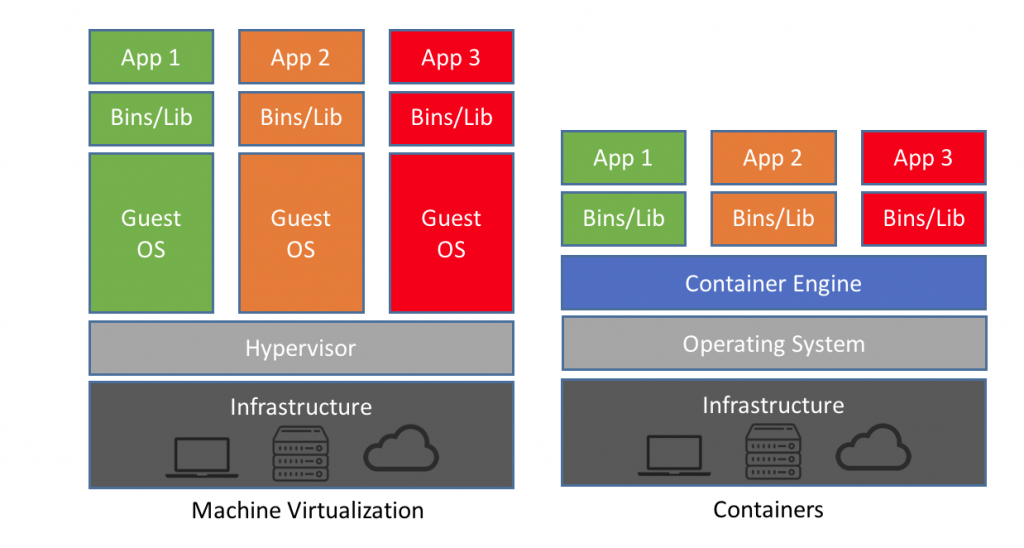
\includegraphics[scale=0.3]{imagenes/03_Estado_del_arte/containers.png}
	\centering
	\caption{Diferencia entre un contenedor y una Máquina Virtual.}
\end{figure}

Entre los \textit{container engines} más populares tenemos \textit{Docker} \cite{docker} y \textit{Podman} \cite{podman}. Recientemente, \textit{Docker} ha sido deprecado en \textit{Kubernetes} (una tecnología para orquestar contenedores ejecutándose en un cluster) debido a problemas de seguridad que presenta su diseño (usa un demonio para funcionar y ejecuta los contenedores con permisos root). \textit{Podman} arregla los problemas que presenta \textit{Docker}, pues no necesita de un demonio para ejecutarse y es \textit{rootless} por tanto es un \textit{engine} más seguro.

\section{Modelos de Machine Learning y Deep Learning}

En esta sección se describirán los modelos de Machine Learning o Deep Learning que se planean usar en los experimentos sobre el dataset. Debemos de tener en cuenta que nos estamos enfrentando a un problema de clasificación, es decir, tenemos que entrenar modelos que intenten predecir un valor discreto \{0, 1\}. El 0 indica que la señal no es de un muón y el 1 indica que sí hay muón registrado en esa señal. Las variables que nos ayudan a predecir son las medidas de la señal en distintos momentos, es una serie temporal. En este proyecto probaré algunos modelos estado del arte en el campo de análisis de series temporales.

\subsection{Concepto básicos}

Algunos de los conceptos básicos sobre Machine Learning o Deep Learning son los siguientes:

\begin{itemize}
	\item \textbf{Dataset}: conjunto de datos que disponemos para entrenar el modelo predictivo. Este dataset se divide en 3 subconjuntos disjuntos, para entrenenar, validar y evaluar el modelo.
	\item \textbf{Training Dataset}: contiene los datos que usaremos para ajustar el modelo.
	\item \textbf{Validation Dataset}: los datos contenidos en este dataset se utilizan para la selección de hiperparámetros más convenientes para entrenar el modelo.
	\item \textbf{Test Dataset}: se utiliza para evaluar la potencia predictiva del modelo.
	\item \textbf{Alto sesgo (high bias)}: esto se produce cuando el poder predictivo del modelo en el conjunto de entrenamiento es malo y por tanto tampoco es capaz de hacer buenas predicciones fuera del conjunto de entrenamiento.
	\item \textbf{Alta variabilidad (high variability)}: esto se produce cuando el modelo se comporta muy bien en el conjunto de entrenamiento, pero funciona muy mal en el conjunto de test (hace predicciones muy malas). Esto es consecuencia del \textit{overfitting}, que se produce porque el modelo se sobreajusta al conjunto de entrenamiento y por tanto no rinde bien en el conjunto de test. Esto suele pasar porque no tenemos datos suficientes para hacer una predicción en condiciones o porque hemos usado un modelo muy complejo.
\end{itemize}

Siempre el conjunto de entrenamiento debe ser mayor que los demás, ya que usar un número muy grande de datos hace que el modelo generado del entrenamiento sea mejor. En los capítulos posteriores explicaré los modelos estado del arte que usaré y los mejores algoritmos de entrenamiento de modelos actuales. También hablaré sobre como podemos evitar el overfitting usando un método muy sencillo llamado regularización.

\subsection{Redes neuronales}

Las redes neuronales son un modelo muy usado para aproximar funciones y en muchos problemas más. Fue inventada en los años 80, pero no era muy usada debido a que no había computadores tan potentes como los de ahora. Gracias a las capacidades de computación modernas, se han podido hacer Redes Neuronales más profundas que ofrecían mejores resultados.\newline

Este modelo de aprendizaje automático se puede usar tanto para regresión lineal (cuando el valor que queremos predecir es continuo) como para regresión logística o clasificación (intentamos predecir un valor discreto que representa la clase a la que pertenece la instancia del dataset). Vamos a pasar a ver cómo funciona este modelo tan popular, empezando por un modelo muy básico.

\begin{figure}[H]
	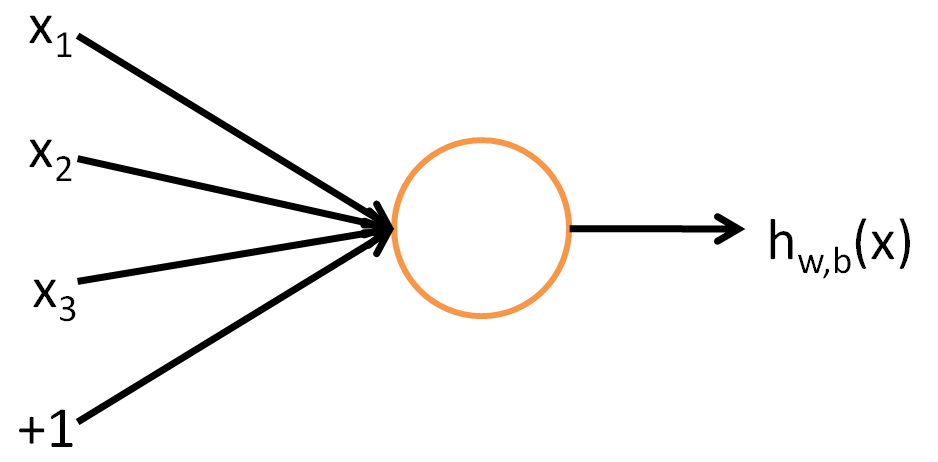
\includegraphics[scale=0.25]{imagenes/03_Estado_del_arte/simplenn.png}
	\centering
	\caption{Red neuronal básica \cite{ng}.}
	\label{fig:simlestnn}
\end{figure}

En la Figura \ref{fig:simlestnn} se puede observar una Red Neuronal muy simple, de hecho este caso específico de red es lo que se llama regresión lineal o logística (dependiendo del rango que tome el valor que intentamos predecir). Una neurona no es más que una función cuya salida es $h_{W,b}(x)=f(W^Tx+b)$, el parámetro $b$ corresponde a las unidades de \textit{bias} y debe ser aprendido al igual que $W$ que representa los pesos. La función $f$ es la función de activación, las más comunes son sigmoide (\ref{eq:sigmoid}), tangente hiperbólica (\ref{eq:tanh}) y RELU (\ref{eq:RELU}). El vector $x$ es el vector de datos, es decir, contiene el dataset. Expresado de otra forma más sencilla, la salida es la siguiente:\newline

$$h_{W,b}=f(W_1 x_1+ W_2 x_2 + W_3 x_3 + b)$$

Las funciones de activación de las que hablé pueden ser las siguientes:

\begin{equation}
	f(x) = \frac{1}{1+e^{-x}}
	\label{eq:sigmoid}
\end{equation}

\begin{equation}
	f(x) = \frac{e^x - e^{-x}}{e^x + e^{-x}}
	\label{eq:tanh}
\end{equation}

\begin{equation}
	f(x) = \max (0, x)
	\label{eq:RELU}
\end{equation}

Con el modelo anterior podríamos predecir un valor o la probabilidad de que una instancia del Dataset pertenezca a una clase u otra (usando por ejemplo la sigmoide que devuelve un valor entre 0 y 1). Ahora que sabemos lo básico, podemos pasar a explicar otra un poco más compleja para comprender como funciona una red neuronal. \newline

\begin{figure}[H]
	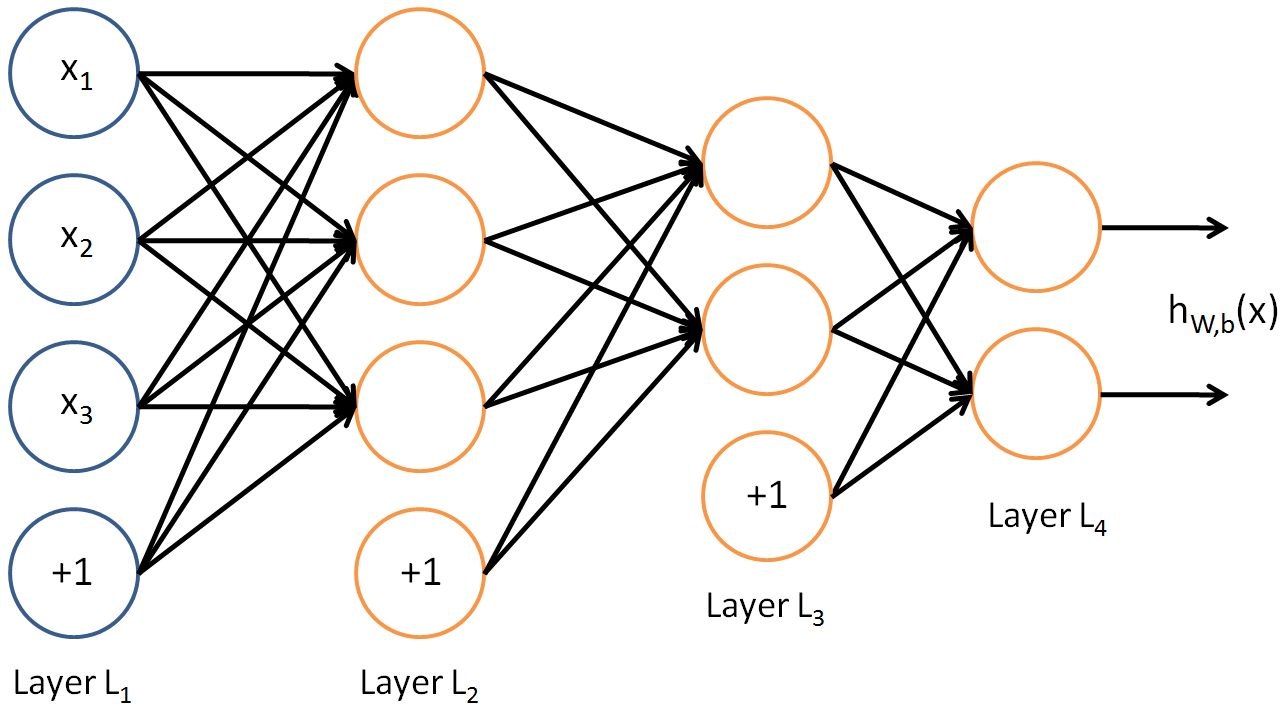
\includegraphics[scale=0.2]{imagenes/03_Estado_del_arte/complexnn.png}
	\centering
	\caption{Red neuronal un poco más compleja \cite{ng}.}
	\label{fig:complexnn}
\end{figure}

En la Figura \ref{fig:complexnn} podemos ver una Red Neuronal más compleja que la anterior. Tanto en esta como en la anterior podemos observar que el tamaño de la entrada en la red es el tamaño de una instancia del dataset + 1 (la unidad de \textit{bias}). El tamaño del output, en un problema de clasificación depende del número de clases que tengamos, en este caso sirve para 2. En este caso, para realizar una predicción deberíamos usar el algoritmo de propagación hacia delante:

\begin{align*}
&a^{(1)} = x^{(i)} \\
&z^{(2)} = W^{(1)}a^{(1)} + b^{(1)} \\
&a^{(2)} = f(z^{(2)}) \\
&z^{(3)} = W^{(2)}a^{(2)} + b^{(2)} \\
&a^{(3)} = f(z^{(3)}) \\
&z^{(4)} = W^{(3)}a^{(3)} + b^{(3)} \\
&h_{W,b}(x) = a^{(4)} = f(z^{(4)})\\
\end{align*}

Una vez obtenido el resultado del algoritmo de propagación hacia delante, podemos obtener la probabilidad de que la instancia pertenezca a cada clase usando \textbf{softmax}:

\begin{align*}
\sigma (z)_j = \frac{e^{z_j}}{\sum^{K}_{k=1} e^{z_k}}
\end{align*}

\subsubsection{Descenso del gradiente}

Anteriormente se ha explicado cómo funciona una red neuronal para predecir, pero ¿Cómo se entrenan para tal objetivo? Primero tenemos que especificar la función que queremos optimizar o dicho de otras palabras, la función que calcula el error en las predicciones y que queremos optimizar. Puede ser el Mean Squared Error (MSE):

\begin{align*}
	&J(W,b;x^{(i)},y^{(i)}) = \frac{1}{m} \sum^m_{i=1} (h_{W,b}(x^{(i)}) - y^{(i)} )^2
\end{align*}

En este caso, el error se calcula como la diferencia entre el valor predecido y el valor correcto. Otra función que podemos usar es la de Cross Entropy (CE):

\begin{align*}
	&J(W,b;x^{(i)},y^{(i)}) = - \frac{1}{m}\left(\sum^m_{i=1} y^{(i)} \cdot \log{h_{W,b}(x^{(i)}})\right)
\end{align*}

El caso específica de CE para dos clases se calcula así:

\begin{align*}
	&J(W,b;x^{(i)},y^{(i)}) = - \frac{1}{m} \left( \sum^m_{i=1} y^{(i)} \cdot \log (h_{W,b}(x^{(i)})) + (1 - y^{(i)}) \cdot \log (1 - h_{W,b}(x^{(i)})) \right)
\end{align*}

Una vez elegida la función de pérdida, debemos optimizarla usando el algoritmo llamado \textit{descenso del gradiente}. Dicho algoritmo actualiza los pesos en cada iteración de la siguiente forma en los modelos básicos de regresión (la red neuronal más básica):

\begin{align*}
	&W_j = W_j - \alpha \frac{\partial}{\partial W_j} J(W,b)\\
	&b = b - \alpha \frac{\partial}{\partial b} J(W,b)\\
\end{align*}

El parámetro $\alpha$ representa el ratio de aprendizaje y es otro parámetro que debemos elegir usando el conjunto de validación. Si es muy alto, el aprendizaje puede fallar y si es muy bajo el entrenamiento tarda un montón en finalizar. Sin embargo, calcular las derivadas parciales en una red neuronal con más capas es un poco más complejo:

\begin{align*}
	&W^{(l)}_{ij} = W^{(l)}_{ij} - \alpha \frac{\partial}{\partial W^{(l)}_{ij}} J(W,b)\\
	&b^{(l)}_i = b^{(l)}_i - \alpha \frac{\partial}{\partial b^{(l)}_i} J(W,b)\\
\end{align*}

Para calcular las derivadas parciales de forma eficiente, se usa el algoritmo de \textit{propagación hacia detrás}:\\

\begin{algorithm}[H]
	\SetAlgoLined
	
	Calcular $a^{(l)}$ $\forall l \in \{2, ..., L\}$ usando el algoritmo de \textit{propagación hacia delante}
	
	Para la capa de salida, calculamos: $\delta^{(L)} = \frac{\partial}{\partial z^{(L)}} \frac{1}{2} || y - h_{W,b}(x) ||^2 = (a^{(L)}- y) \odot f'(z^{(L)})$
	
	\For{$l \in \{L-1, ..., 2\}$}{
		\nonl $\delta^{(l)} = ((W^{(l)})^T \delta^{(l+1)}) \odot f'(z^{(l)})$
	}
	
	Calcular las derivadas parciales:\\
	\nonl $\frac{\partial}{\partial W^{(l)}} = \delta^{(l+1)}(a^{(l)})^T$\\
	\nonl $\frac{\partial}{\partial b^{(l)}} = \delta^{(l+1)}$
	
	\caption{Backpropagation Algorithm}
\end{algorithm}

\subsection{Mejoras para el modelo de Red Neuronal}

\subsection{Autoencoders}

\subsection{Redes Neuronales Convolucionales}
